\documentclass[12pt,letterpaper]{report}

% Paquetes necesarios
\usepackage[spanish]{babel}
\usepackage[utf8]{inputenc}
\usepackage{graphicx}
\usepackage{hyperref}
\usepackage{color}
\usepackage{xcolor}
\usepackage{fancyhdr}
\usepackage{tcolorbox}
\usepackage{enumerate}
\usepackage{listings}
\usepackage{geometry}
\usepackage{wrapfig}
\usepackage{mdframed}
\usepackage{lipsum}
\usepackage{parskip} 
\usepackage{float}

% Configuración de párrafos
\setlength{\parindent}{0pt}  % Elimina la indentación de todos los párrafos
\setlength{\parskip}{1em}    % Añade espacio entre párrafos

% Configuración de geometría
\geometry{
    top=2.5cm,
    bottom=2.5cm,
    left=3cm,
    right=3cm,
    headheight=15pt
}

% Configuración de colores
\definecolor{liese-blue}{RGB}{0, 82, 155}
\definecolor{warning}{RGB}{255, 127, 0}
\definecolor{tip-green}{RGB}{46, 139, 87}
\definecolor{note-blue}{RGB}{70, 130, 180}

% Configuración de listings
\lstset{
    basicstyle=\ttfamily\small,
    breaklines=true,
    frame=single,
    numbers=left,
    numberstyle=\tiny,
    keywordstyle=\color{blue},
    commentstyle=\color{green!60!black},
    stringstyle=\color{orange},
    showstringspaces=false
}

% Definición de entornos personalizados
\newenvironment{tip}
    {\begin{mdframed}[linecolor=tip-green,linewidth=2pt,backgroundcolor=tip-green!10]
    \textbf{Consejo:}\par}
    {\end{mdframed}}

\newenvironment{note}
    {\begin{mdframed}[linecolor=note-blue,linewidth=2pt,backgroundcolor=note-blue!10]
    \textbf{Nota:}\par}
    {\end{mdframed}}

\newenvironment{warning-box}
    {\begin{mdframed}[linecolor=warning,linewidth=2pt,backgroundcolor=warning!10]
    \textbf{Advertencia:}\par}
    {\end{mdframed}}

% Configuración de hipervínculos
\hypersetup{
    colorlinks=true,
    linkcolor=liese-blue,
    filecolor=liese-blue,
    urlcolor=liese-blue,
}

% Configuración de encabezado y pie de página
\pagestyle{fancy}
\fancyhf{}
\rhead{LIESE}
\lhead{Manual de Usuario}
\rfoot{Página \thepage}

% Inicio del documento
\begin{document}

\begin{titlepage}
    \centering
    \vspace*{1cm}
    
    % Logo UNAM
    
\includegraphics[width=0.1\textwidth]{images/unam.png}\\[1.2cm]
    
    {\Large División de Ingeniería Eléctrica}
    
    
    {\Huge\bfseries Manual de Usuario\\[0.5cm] 
    Sitio Web LIESE\\[1.5cm]}
    
    % Logo LIESE
    
\includegraphics[width=0.2\textwidth]{images/logo.png}\\[1.5cm]
    
    {\Large\itshape Laboratorio de Instrumentación Espacial\\[0.3cm]
    Universidad Nacional Autónoma de México\\[1cm]}
    
    {\large Autor:\\
    Jorge Eithan Treviño Selles\\[0.3cm]
    Desarrollador del Sitio Web}\\[1cm]
    
    {\large Primera Edición\\
    \today}
    
    \vfill
    
    {\small © 2025 LIESE - División de Ingeniería Eléctrica, Facultad de Ingeniería, UNAM.}
\end{titlepage}
\newpage

\tableofcontents
\newpage

\chapter{Introducción}

\begin{note}
Este manual está diseñado para guiar a los administradores del sitio web del LIESE en la gestión y actualización del contenido. No se requieren conocimientos técnicos de programación o desarrollo web para realizar estas tareas.
\end{note}

\section{Acerca del LIESE}
El Laboratorio de Instrumentación Espacial (LIESE) es una unidad de investigación de la División de Ingeniería Eléctrica (DIE) de la Facultad de Ingeniería de la UNAM dedicada al desarrollo de tecnología espacial y la formación de recursos humanos en el área. Nuestro sitio web es la ventana principal al mundo de nuestras actividades, investigaciones y logros.

\section{Propósito del Sitio Web}
El sitio web del LIESE es la plataforma oficial de comunicación que cumple varios objetivos fundamentales:
\begin{itemize}
    \item Presentar el trabajo y los logros del laboratorio en instrumentación espacial
    \item Dar visibilidad a los líderes de proyecto y sus líneas de investigación
    \item Mantener un calendario actualizado de eventos y actividades académicas
    \item Difundir artículos y publicaciones científicas relevantes
    \item Compartir información sobre los proyectos actuales y sus avances
    \item Comunicar las actividades y colaboraciones del laboratorio
    \item Publicar oportunidades de colaboración y desarrollo académico
    \item Facilitar la vinculación con instituciones y posibles patrocinadores
\end{itemize}

\section{Estructura del Sitio}
El sitio web está organizado en las siguientes secciones principales:

\subsection{Inicio}
\begin{itemize}
    \item Sección "¿Quiénes somos?" con información del LIESE y su director
    \item Áreas de investigación con tarjetas informativas
    \item Sección de socios y colaboradores
    \item Sección de contacto con ubicación y redes sociales
    \item Botones de acceso rápido a Eventos y Actividades
\end{itemize}

\subsection{Líderes de Proyecto}
\begin{itemize}
    \item Perfiles de los líderes de investigación
    \item Áreas de especialización
    \item Información de contacto
    \item Proyectos actuales
\end{itemize}

\subsection{Eventos}
\begin{itemize}
    \item Calendario de eventos próximos
    \item Detalles de cada evento
    \item Fecha y ubicación
    \item Descripción del evento
\end{itemize}

\subsection{Artículos}
\begin{itemize}
    \item Publicaciones científicas
    \item Reportes de investigación
    \item Avances de proyectos
    \item Referencias y enlaces
\end{itemize}

\subsection{Proyectos}
\begin{itemize}
    \item Proyectos actuales con trabajo de tesis
    \item Descripción de cada proyecto
    \item Líder del proyecto
    \item Estado y avances
\end{itemize}

\subsection{Actividades}
\begin{itemize}
    \item Vista general de todas las actividades
    \item Sección de eventos
    \item Sección de noticias
    \item Sección de proyectos
    \item Sección de artículos
\end{itemize}

\subsection{Oportunidades}
\begin{itemize}
    \item Formulario de solicitud con autenticación de dos factores
    \item Campos del formulario:
        \begin{itemize}
            \item Nombre completo
            \item Correo electrónico (requiere verificación)
            \item Tipo de oportunidad
            \item Mensaje o propuesta
            \item Documentos adjuntos
        \end{itemize}
    \item Sistema de verificación por correo electrónico
    \item Seguimiento del estado de la solicitud
\end{itemize}

\begin{note}
El sistema de autenticación de dos factores (2FA) para oportunidades funciona de la siguiente manera:
\begin{enumerate}
    \item El usuario llena el formulario de solicitud
    \item Se envía un correo de verificación a la dirección proporcionada
    \item El usuario debe hacer clic en el enlace de verificación
    \item Solo después de la verificación, la solicitud se registra en el sistema
\end{enumerate}
Este proceso asegura que las solicitudes provengan de direcciones de correo válidas y ayuda a prevenir spam.
\end{note}

\section{¿Qué puedo hacer como administrador?}
Como administrador del sitio, usted tendrá acceso a un conjunto completo de herramientas para gestionar el contenido:

\subsection{Gestión de Contenido}
\begin{itemize}
    \item Crear, editar y eliminar artículos
    \item Publicar y actualizar noticias
    \item Gestionar eventos y calendario
    \item Actualizar información de miembros
    \item Administrar solicitudes de oportunidades
\end{itemize}

\subsection{Gestión de Medios}
\begin{itemize}
    \item Subir y organizar imágenes
    \item Administrar fotos de artículos, actividades, eventos y proyectos
    \item Administrar documentos adjuntos
\end{itemize}

\subsection{Gestión de Usuarios}
\begin{itemize}
    \item Revisar solicitudes de registro
    \item Gestionar permisos de usuarios
    \item Monitorear actividad de usuarios
    \item Mantener la seguridad del sitio
\end{itemize}

\begin{tip}
Como administrador, usted es responsable de mantener la calidad y actualidad del contenido. Recuerde que el sitio web es la cara pública del LIESE y debe reflejar nuestra excelencia académica y profesionalismo.
\end{tip}

\section{Flujo de Trabajo Típico}
Un día típico como administrador del sitio puede incluir:

\begin{enumerate}
    \item Revisar y responder solicitudes pendientes
    \item Actualizar calendario de eventos
    \item Publicar noticias relevantes
    \item Actualizar información de miembros
    \item Mantener actualizada la sección de oportunidades
    \item Responder consultas de usuarios
\end{enumerate}

\begin{warning-box}
Siempre verifique la información antes de publicarla. Una vez publicada, será visible para todo el mundo y representa al LIESE oficialmente.
\end{warning-box}

\chapter{Acceso al Panel de Administración}

\section{Iniciar Sesión}
\begin{enumerate}
    \item Visite \url{http://liese.unam.mx/admin}
    \item Ingrese su nombre de usuario y contraseña
    \item Haga clic en "Iniciar sesión"
\end{enumerate}

\begin{figure}[H]
    \centering
    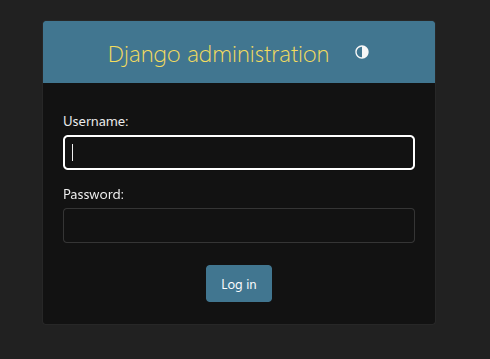
\includegraphics[width=0.6\textwidth]{images/login.png}
    \caption{Pantalla de inicio de sesión del panel de administración}
\end{figure}

\section{Vista General del Panel}
Al ingresar, encontrará un tablero con las siguientes secciones principales:
\begin{itemize}
    \item Artículos
    \item Eventos
    \item Miembros
    \item Noticias
    \item Solicitudes de Oportunidades
\end{itemize}

\begin{figure}[H]
    \centering
    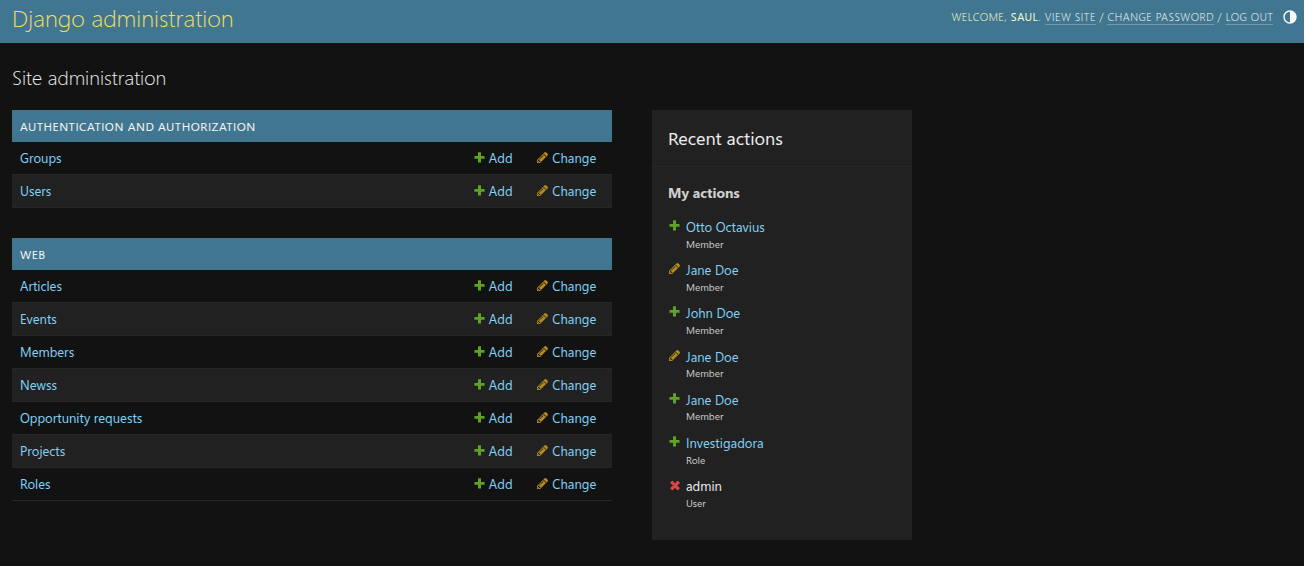
\includegraphics[width=0.8\textwidth]{images/panel.png}
    \caption{Panel principal del administrador}
\end{figure}

\chapter{Gestión de Contenido}

\section{Artículos}
\subsection{Agregar un Nuevo Artículo}
\begin{enumerate}
    \item En el panel, haga clic en  Articles"
    \item Haga clic en el botón "ADD ARTICLE +"
    \item Complete los siguientes campos:
        \begin{itemize}
            \item Title
            \item Content
            \item Published (si desea que el artículo esté visible inmediatamente)
            \item Publication Date
            \item Author
            \item Picture (opcional)
            \item Document (opcional)
        \end{itemize}
    \item Haga clic en "Guardar"
\end{enumerate}

\begin{figure}[H]
    \centering
    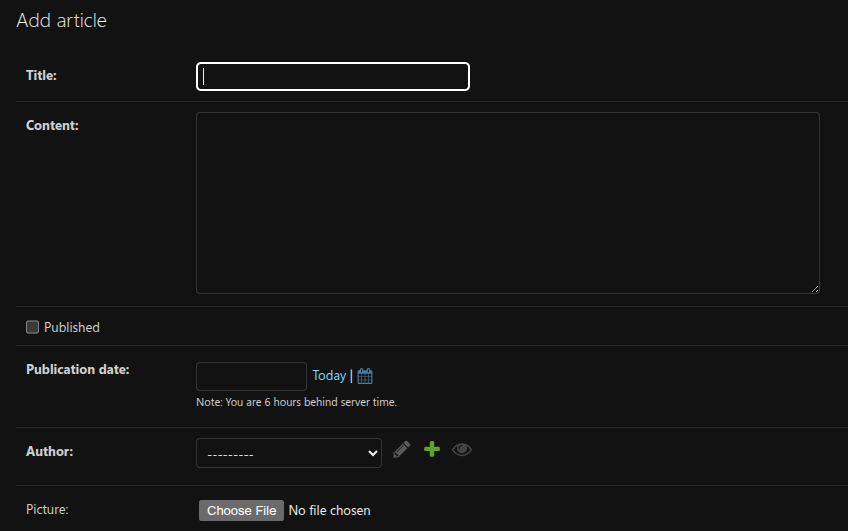
\includegraphics[width=0.8\textwidth]{images/article.png}
    \caption{Formulario para agregar un nuevo artículo}
\end{figure}

\section{Eventos}
\subsection{Crear un Nuevo Evento}
\begin{enumerate}
    \item En el panel, seleccione "Evento"
    \item Haga clic en " ADD EVENTO +"
    \item Complete la información:
        \begin{itemize}
            \item Title
            \item Description
            \item Start Date and Time
            \item End Date and Time
            \item Location
            \item Category
            \item Image (opcional)
            \item Published (si desea que el evento esté visible inmediatamente)
            \item Created By
        \end{itemize}
    \item Haga clic en "Save and add another" para agregar más eventos o "Save" para finalizar
\end{enumerate}



\section{Miembros}
\subsection{Agregar un Nuevo Miembro}
\begin{enumerate}
    \item Vaya a la sección "Members"
    \item Haga clic en "ADD MEMBER +"
    \item Complete los campos:
        \begin{itemize}
            \item First Name
            \item Last Name
            \item Email
            \item Phone
            \item Country
            \item Position
            \item Description
            \item Date joined
            \item Roles
            \item Is leader (si es líder de proyecto)
            \item Active
            \item Image (opcional)
            \item LinkedIn (opcional)
            \item Admin (si tendrá acceso al panel de administración)
            \item Created By (si desea registrar quién creó el miembro)
            \item Username
            \item Password
        \end{itemize}
    \item Haga clic en "Save and add another" para agregar más eventos o "Save" para finalizar
\end{enumerate}

\begin{figure}[H]
    \centering
    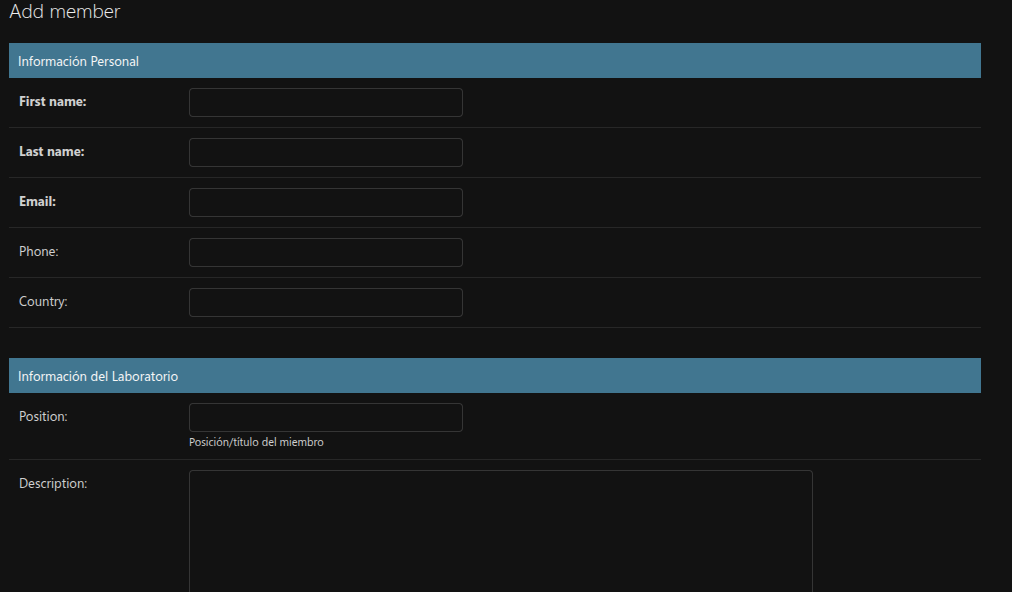
\includegraphics[width=0.8\textwidth]{images/add_user.png}
    \caption{Formulario para agregar un nuevo miembro}
\end{figure}

\section{Noticias}
\subsection{Publicar una Nueva Noticia}
\begin{enumerate}
    \item Acceda a la sección "Newss"
    \item Haga clic en "ADD NEWS +"
    \item Rellene los campos:
        \begin{itemize}
            \item Title
            \item Content
            \item Published (si desea que la noticia esté visible inmediatamente)
            \item Publication Date
            \item Author
        \end{itemize}
    \item Haga clic en "Save and add another" para agregar más eventos o "Save" para finalizar
\end{enumerate}

\begin{figure}[H]
    \centering
    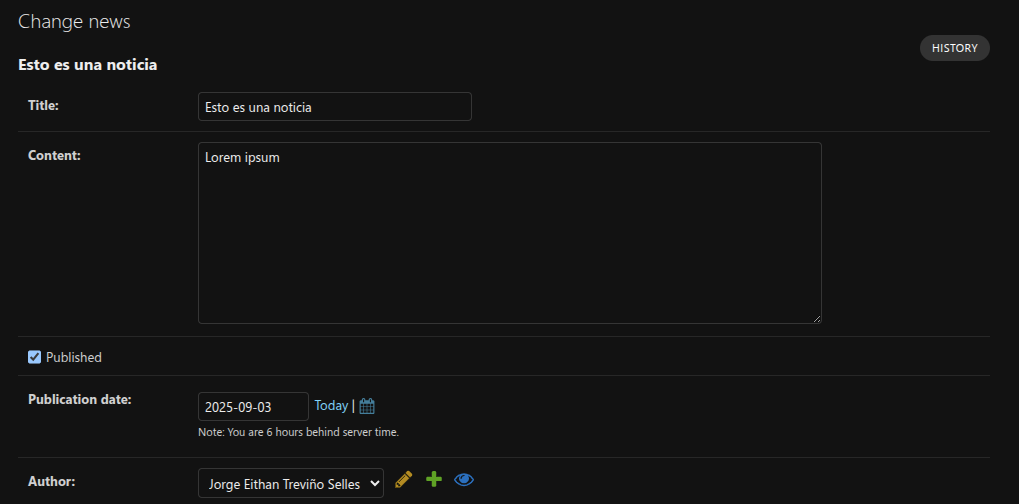
\includegraphics[width=0.8\textwidth]{images/news.png}
    \caption{Formulario para agregar una nueva noticia}
\end{figure}

\section{Projects}
\subsection{Publicar un Nuevo Proyecto}
\begin{enumerate}
    \item Acceda a la sección "Projects"
    \item Haga clic en "ADD PROJECT +"
    \item Rellene los campos:
        \begin{itemize}
            \item Name
            \item Description
            \item Start date
            \item End date
            \item Active
            \item Image (opcional)
        \end{itemize}
        \item Agregue a los miembros del proyecto, incluyendo al líder del proyecto.
    \item Haga clic en "Guardar"
\end{enumerate}

\begin{figure}[H]
    \centering
    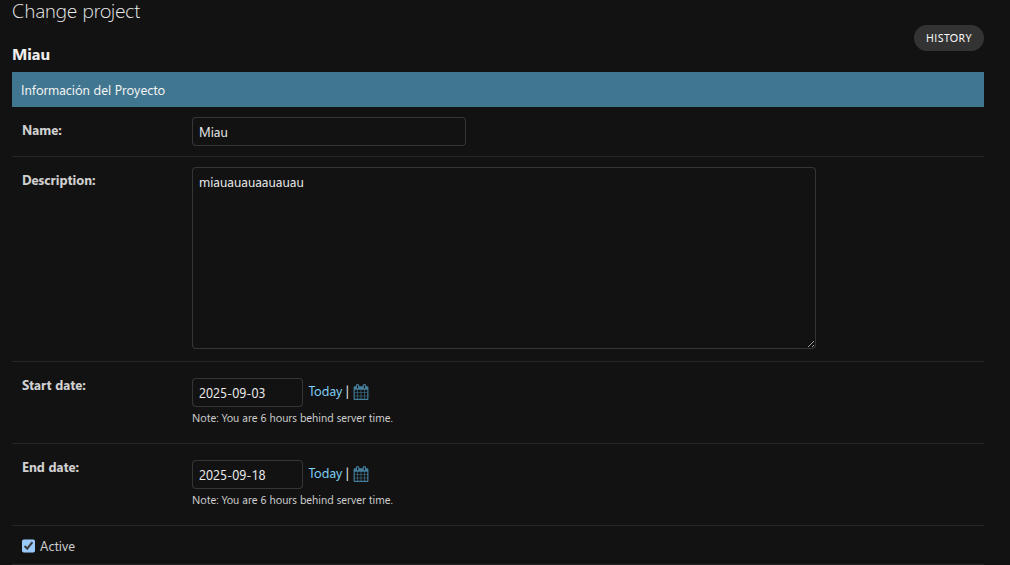
\includegraphics[width=0.8\textwidth]{images/projects.png}
    \caption{Formulario para agregar un nuevo proyecto}
\end{figure}

\section{Roles}
\subsection{Administrar roles}
\begin{enumerate}
    \item En el panel, haga clic en "Roles"
    \item Verá una lista de todas los roles creados
    \item Si desea agregar un rol, haga clic en "ADD ROLE +"
    \item Escriba el nombre y descripción del rol
    \item Asigne el rol dentro de la pestaña "Members"
\end{enumerate}

\begin{figure}[H]
    \centering
    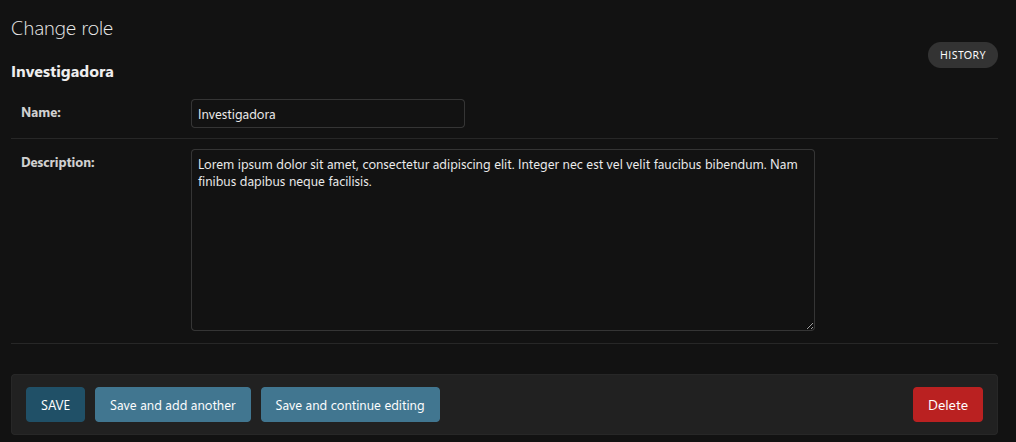
\includegraphics[width=0.8\textwidth]{images/role.png}
    \caption{Lista de roles y formulario para agregar un nuevo rol}
\end{figure}



\chapter{Gestión de Solicitudes}

\section{Solicitudes de Oportunidades}
\subsection{Revisar Solicitudes}
\begin{enumerate}
    \item En el panel, haga clic en "Opportunity requests"
    \item Verá una lista de todas las solicitudes recibidas
    \item Puede filtrar por:
        \begin{itemize}
            \item Nombre
            \item Correo electrónico
            \item Tipo de oportunidad
            \item Verificado (si el usuario ha verificado su correo)
            \item Timestamp
        \end{itemize}
    \item Haga clic en una solicitud para ver lo que escribió el usuario al momento de aplicar.
\end{enumerate}

\begin{figure}[H]
    \centering
    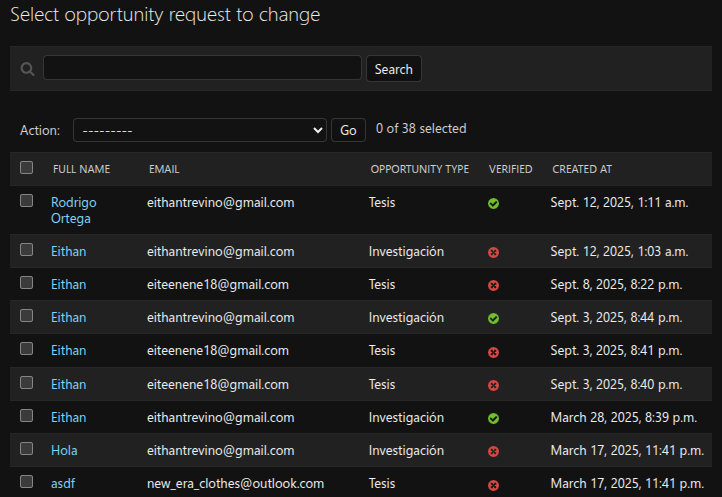
\includegraphics[width=0.8\textwidth]{images/opportunity_requests.png}
    \caption{Lista de solicitudes de oportunidades}
\end{figure}



\chapter{Consejos y Mejores Prácticas}

\section{Imágenes}
\begin{tcolorbox}[colback=blue!5,colframe=liese-blue]
\textbf{Recomendaciones para imágenes:}
\begin{itemize}
    \item Use imágenes de alta calidad pero optimizadas para web
    \item Tamaño recomendado para imágenes destacadas: 1200 x 630 píxeles
    \item Formatos aceptados: JPG, PNG
    \item Tamaño máximo de archivo: 5MB
\end{itemize}
\end{tcolorbox}

\section{Contenido}
\begin{tcolorbox}[colback=blue!5,colframe=liese-blue]
\textbf{Consejos para el contenido:}
\begin{itemize}
    \item Escriba títulos claros y descriptivos
    \item Use párrafos cortos para mejor legibilidad
    \item Incluya palabras clave relevantes
    \item Revise la ortografía antes de publicar
\end{itemize}
\end{tcolorbox}

\chapter{Solución de Problemas}

\section{Problemas Comunes}
\begin{enumerate}
    \item \textbf{No puedo iniciar sesión}
        \begin{itemize}
            \item Verifique que su nombre de usuario y contraseña sean correctos
            \item Asegúrese de que las mayúsculas/minúsculas sean correctas
            \item Si olvidó su contraseña, use la opción "¿Olvidó su contraseña?"
        \end{itemize}
    
    \item \textbf{No puedo subir una imagen}
        \begin{itemize}
            \item Verifique el tamaño del archivo
            \item Asegúrese de que el formato sea compatible
            \item Intente optimizar la imagen
        \end{itemize}
    
    \item \textbf{Los cambios no se ven reflejados}
        \begin{itemize}
            \item Actualice la página con Ctrl+F5
            \item Verifique que guardó los cambios
            \item Espere unos minutos y vuelva a intentar
        \end{itemize}
\end{enumerate}

\section{Contacto de Soporte}
Si encuentra algún problema que no puede resolver:
\begin{tcolorbox}[colback=warning!15,colframe=warning]
\begin{itemize}
    \item Correo de soporte: eithantrevino@gmail.com
    \item Teléfono: 5581484013
\end{itemize}
\end{tcolorbox}

\end{document}